\documentclass{webofc}
\usepackage[varg]{txfonts}   % Web of Conferences font

\usepackage[T2A]{fontenc} % указывает внутреннюю кодировку TeX
\usepackage[english]{babel}   %% загружает пакет многоязыковой вёрстки
\usepackage{color}
\usepackage{tasks}
\settasks {counter-format=(tsk[r])}
%\usepackage{exsheets}
\usepackage{array,graphicx,caption,paralist}
\usepackage{floatflt,wrapfig}
\newcommand{\er}{\textmd{EXPERTroot}}

\newcommand{\red}[1]{\textcolor{red}{#1}}

\begin{document}
\title{Timing properties of the NeuRad detector prototype}

\author{\firstname{I.} \lastname{Muzalevsky}\inst{1,3,4}\fnsep\thanks{\email{ivanmuzalevskij@gmail.com}} \and
	\firstname{V.} \lastname{Chudoba}\inst{1,3}\fnsep\thanks{\email{chudoba@jinr.ru}} \and
	\firstname{A.} \lastname{Bezbakh}\inst{1,3} \and
	\firstname{S.} \lastname{Belogurov}\inst{1} \and
	\firstname{I.} \lastname{Mukha}\inst{5} \and
	\firstname{O.} \lastname{Kiselev}\inst{5} \and
	\firstname{A.} \lastname{Fomichev}\inst{1} \and
	\firstname{S.} \lastname{Krupko}\inst{1} \and
	\firstname{R.} \lastname{Slepnev}\inst{1} \and
	\firstname{D.} \lastname{Kostyleva}\inst{5} \and
	\firstname{A.} \lastname{Gorshkov}\inst{1} \and
	\firstname{E.} \lastname{Ovcharenko}\inst{2} \and
	\firstname{V.} \lastname{Schetinin}\inst{2} \and \red{who?}
	 \ for the EXPERT/Super-FRS Experiment Collaboration
	% etc.
}
\institute{
	FLNR JINR Dubna, Russia; 
	\and
	Laboratory of Information Technologies, JINR, Dubna, Russia
	\and
	Silesian University in Opava, Czech Republic;
	\and
	Dubna State University, Russia;
	\and
	GSI Helmholtzzentrum, Darmstadt
}
\abstract{%
%	\color{red}
	One of the subtopics of the SuperFRS Experiment Collaboration, being part of NUSTAR@FAIR, is investigation of properties of light exotic nuclei using EXPERT setup.
	One of its modules, the NeuRad detector, is intended for registration of neutrons emitted by investigated nuclei.
	Present work is dedicated to study of the timing properties of the NeuRad detector prototype. Timing properties of the measured and simulated signals have been studied using digital processing algorithms. Obtained results allow better understanding of the processes in the scintillator fibers coupled to the multi-anode PMT.
}
%
\maketitle
%
%\color{red}
\section{Introduction}
Properties of exotic nuclei represent one of the most important fields in modern nuclear physics.
Such uncommon nuclei are characterized by large excess of neutrons or protons and are located far from the nuclear stability. As far as the binding energy decreases, one may observe the transition from the discrete spectra to nuclear resonances with many overlapping states and, as a consequence, such unique phenomena as neutron halo, soft mode of dipole excitation and others could be observed. Moreover, new decay channels, including many-body, are becoming open \cite{ufn}.

As far as exotic nuclei are unstable one meets a problem how to produce them.
One of the most developed facility for their production by separation in-flight will be fragment separator Super-FRS at FAIR (Facility for Antiproton and Ion Research) \cite{diplom}. Project EXPERT (EXotic Particle Emission and Radioactivity by Tracking \cite{IMexpert}) dedicated to study of properties of exotic nuclei is a part of scientific program of the Super-FRS Experiment Collaboration. \red{dirtyEXPERT} setup consists of five modules each of which is intended to detect different decay products \cite{tdr}.
These modules may be enumerated as:
\begin{inparaenum}[(i)]
	\item Radiation-hard silicon strip detector (SSD) for Time-of-Flight and triggering.
	\item Microstrip silicon ($\mu$Si) tracking detectors.
	\item The gamma-ray and light particles detector system GADAST (GAmma-ray Detectors Around Secondary Target).
	\item The OTPC (Optical Time Projection Chamber) for radioactivity studies by the implantation-decay method.
	\item The NeuRad (Neutron Radioactivity) fine-resolution neutron detector.
\end{inparaenum}

Moreover, the EXPERTroot framework \cite{er} for simulations of the experiments and processing of the experimental data and the software for simulation of theoretical distributions is indissociable part of the project.
%Additional important part of the EXPERT project is a framework for simulations of the experiments and processing of the experimental data. For this purpose a framework EXPERTroot \cite{er} has been developed.
%%EXPERTroot is a framework for Monte-Carlo simulations of detector responses, event reconstruction and EXPERT experiment analysis.
This paper is dedicated to study of the timing properties of the NeuRad detector prototype.
%All necessary methods of data processing and simulation were implemented into the EXPERTroot.

\section{The NeuRad detector}

Neutron detector NeuRad is aimed at providing precise information on angular correlations between neutrons and heavy fragment emitted in the decay of a nucleus of interest. The heavy fragment will be identified by Super-FRS beam diagnostic system whereas trajectories of a heavy fragment and neutrons will be reconstructed by an array of the $\mu$Si detectors and the NeuRad detector respectively. 
This information will be used to determine the decay energy of the nucleus of interest and its lifetime.

NeuRad will be constructed from a large number of scintillating fibers ($\approx$10000 units). Each fiber will have a square cross section of 3$\times$3\,mm$^2$ and the length of 1\,m. Scintillating fibers will be grouped into bundles fitting the photosensors e.g. multi-anode PMTs (MAPMTs).
The neutrons penetrating into the bundles will undergo different interaction processes, but the most important one for the neutron registration will be the elastic scattering on protons. In such a case recoil proton will induce a scintillation light inside the fiber. 
The light emitted within the full reflection angle travels to the MAPMTs located at the both ends of the fiber.
MAPMTs will be mounted to the bundles so that the area of each pixel will completely overlap the frontal surface of one fiber.

%\begin{figure}[h]
%	\center{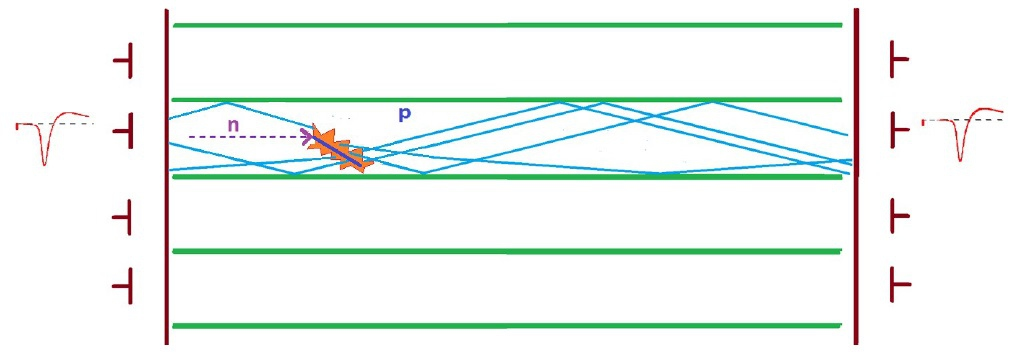
\includegraphics[width=0.8\linewidth]{neurad.png}}
%	\caption{Operational principle of the NeuRad. Each scintillating fiber will be coupled to one pixel of the MAPMT. The neutron beam will penetrate through the frontal MAPMTs.}
%	\label{ris:neuradPrinciple}
%\end{figure}

In the course of planned experiments, NeuRad will be placed in 28\,m downstream of the secondary target so that the fibers will be oriented along the beam direction \cite{report}.
% see Fig.\ref{ris:neuradPrinciple}. 
This is planned in order to provide sufficient efficiency of the detection and fine position resolution for neutrons with energies 200-800\,MeV in the lab frame.
With such a configuration the total angular acceptance of the detector will be about 12\,mrad.
%This number is determined by the low transversal momentum of the neutrons expected in decays with energies in the range of 0.1-100\,keV.
Such value is sufficient to register the low transversal momenta of the neutrons expected in decays with energies in the range of 0.1-100\,keV.

In the case of a single scattering of the neutron inside the Neurad, the position of the fired fiber or the cluster of neighboring fibers gives information about transversal coordinates of the interaction point. Time stamps of the signals from both MAPMTs allow to derive the longitudinal position of the energy deposit and time-of-flight, which is used for the determination of the neutron kinetic energy. 

If several  fibers are fired due to the neutron re-scattering or distribution of the energy deposited by the recoil proton, the first interaction point may be reconstructed by searching for an earliest signal in the upstream MAPMT. Besides, timing information may be used in more sophisticated analysis of the events with multiple hits.

\section{Test of NeuRad timing properties}

The first investigation aimed at obtaining the timing characteristics of the NeuRad detector was conducted recently in Flerov Laboratory of Nuclear Reactions JINR, Dubna. The NeuRad prototype was used for these test measurements. The sensitive part of the prototype was a bundle of 256 optical fibers made of scintillator plastic BCF-12 \cite{crystals}. 
Each fiber was covered with white acrylic paint in the first layer and black aerosol paint in the second one for light insulation and had a cross section of 3$\times$3\,mm$^2$ and a length of 25\,cm. Two MAPMTs H9500 \cite{hm} were mounted to both sides of the bundle. To improve this connection, an optical grease was used.

\begin{figure}[h]
	\centering
	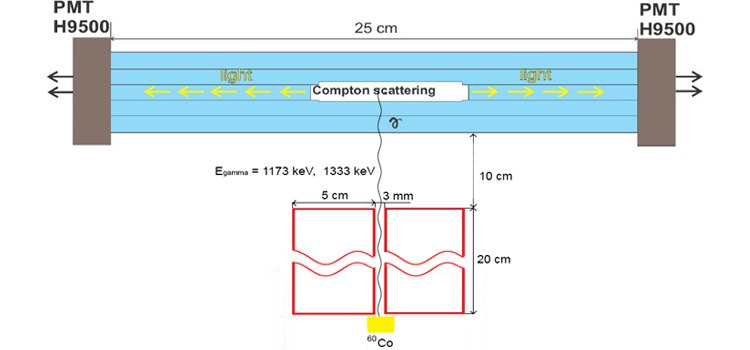
\includegraphics[width=0.7\linewidth]{NeuRadexperiment.png}
	\captionof{figure}{Scheme of measurements with the NeuRad prototype. The prototype was irradiated by a collimated $\gamma$-source $^{60}$Co.
	The gamma rays were focused at the geometrical center of the prototype and signals were collected by a couple of H9500 MAPMTs.	
}
\label{ris:neuradexp}
\end{figure}

This prototype was irradiated by collimated gamma beam with energies $E^{(1)}_{\gamma}$=1173\,keV and $E^{(2)}_{\gamma}$=1333\,keV emitted by $^{60}$Co as showed in Fig.\ref{ris:neuradexp}. Signals obtained from the MAPMTs were collected by the DRS4 evaluation board (12 bit at 5 GS/s) and
%their were
saved for each detected event.

\section{Simulations and data processing}

Simulation and data processing were performed within the \er\, framework.
The geometry created within \er\ and shown in Fig.\,\ref{ris:sim}a) was used for the MC simulations.
Particle transport through the setup was performed using the GEANT4 \cite{geant4} classes.
Obtained energy deposits were converted with use of the \er\ digitizing algorithms into the MAPMT anode pulses.
Each pulse was calculated as a sum of single photoelecton pulses taking into account the following parameters and effects: light output of the scintillating fiber; efficiency of the light trapping into the fiber due to total internal reflection; scintillation decay time; light attenuation along the fiber; light collection increase near the ends of the fiber; light losses at the optical interface; MAPMT quantum efficiency; single photoelectron amplitude spectrum, pulse shape, and spread of the avalanche transition time through the dynode system; cross-talk as a probability of the single photoelecton avalanche developing in the neighboring pixel.
Certain effects were not taken into account: any dependence of the pulse shape on the amplitude; cross-talk as the charge sharing of a single photoelectron avalanche between two or more anodes; partial collection of light after diffuse scattering at the fiber faces; electronic noises; pulse shape distortion in the readout line. Most of the parameters for the simulations were taken from the data-sheets of the fibers and MAPMT.  Only the single photoelectron pulse shape was fitted to the experimental data. The simulated pulse shapes had the same format as in the experimental data.

\begin{figure}[h]
	\begin{minipage}[h]{0.25\linewidth}
		\center{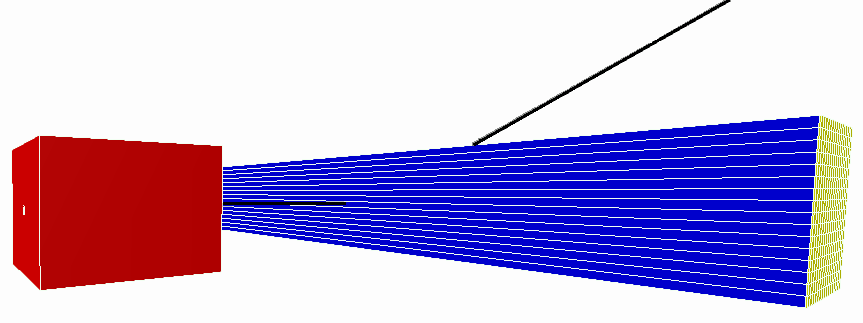
\includegraphics[width=1\linewidth]{sim.png}} a) \\
	\end{minipage}
	\hfill
	\begin{minipage}[h]{0.35\linewidth}
		\center{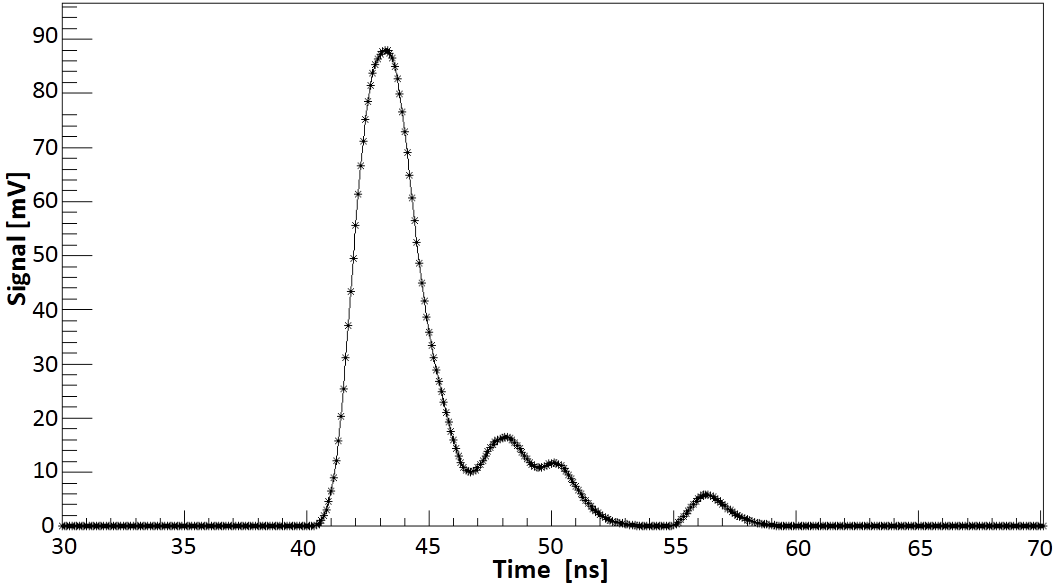
\includegraphics[width=1\linewidth]{simSignal1.png}} b) \\
	\end{minipage}
	\hfill
	\begin{minipage}[h]{0.35\linewidth}
		\center{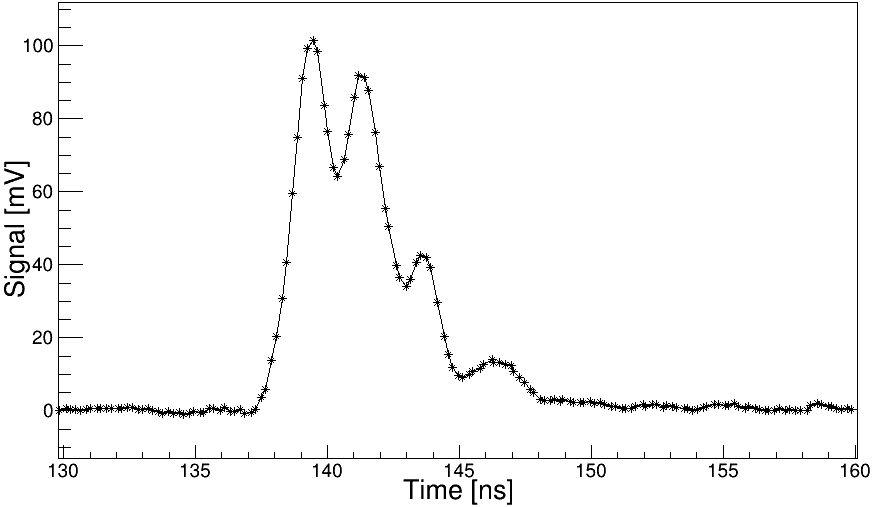
\includegraphics[width=1\linewidth]{originalsignalform.png}} c) \\
	\end{minipage}
	\caption{a) Simulations within the \er. Prototype and collimator are depicted in blue, red colors respectively. The trajectory of the gamma particle is colored in yellow. b) Typical MAPMT's anode output signal form obtained in simulations c) Typical signal form obtained in measurements.}
	\label{ris:sim}
\end{figure}
Typical pulses obtained in simulations and measurements turned out qualitatively similar and are shown in Fig.\ref{ris:sim}b) and Fig.\ref{ris:sim}c) respectively. However, there is a clear difference between the simulated and recoded experimental pulses. In the recorded ones one can notice a kind of low-amplitude afterpulses. Those can be due to several reasons, e.g. stray capacity discharge and influence of the readout line bandwidth, which manifests itself in the damped oscillations caused by the sharp leading edge.

\begin{figure}
	\centering
	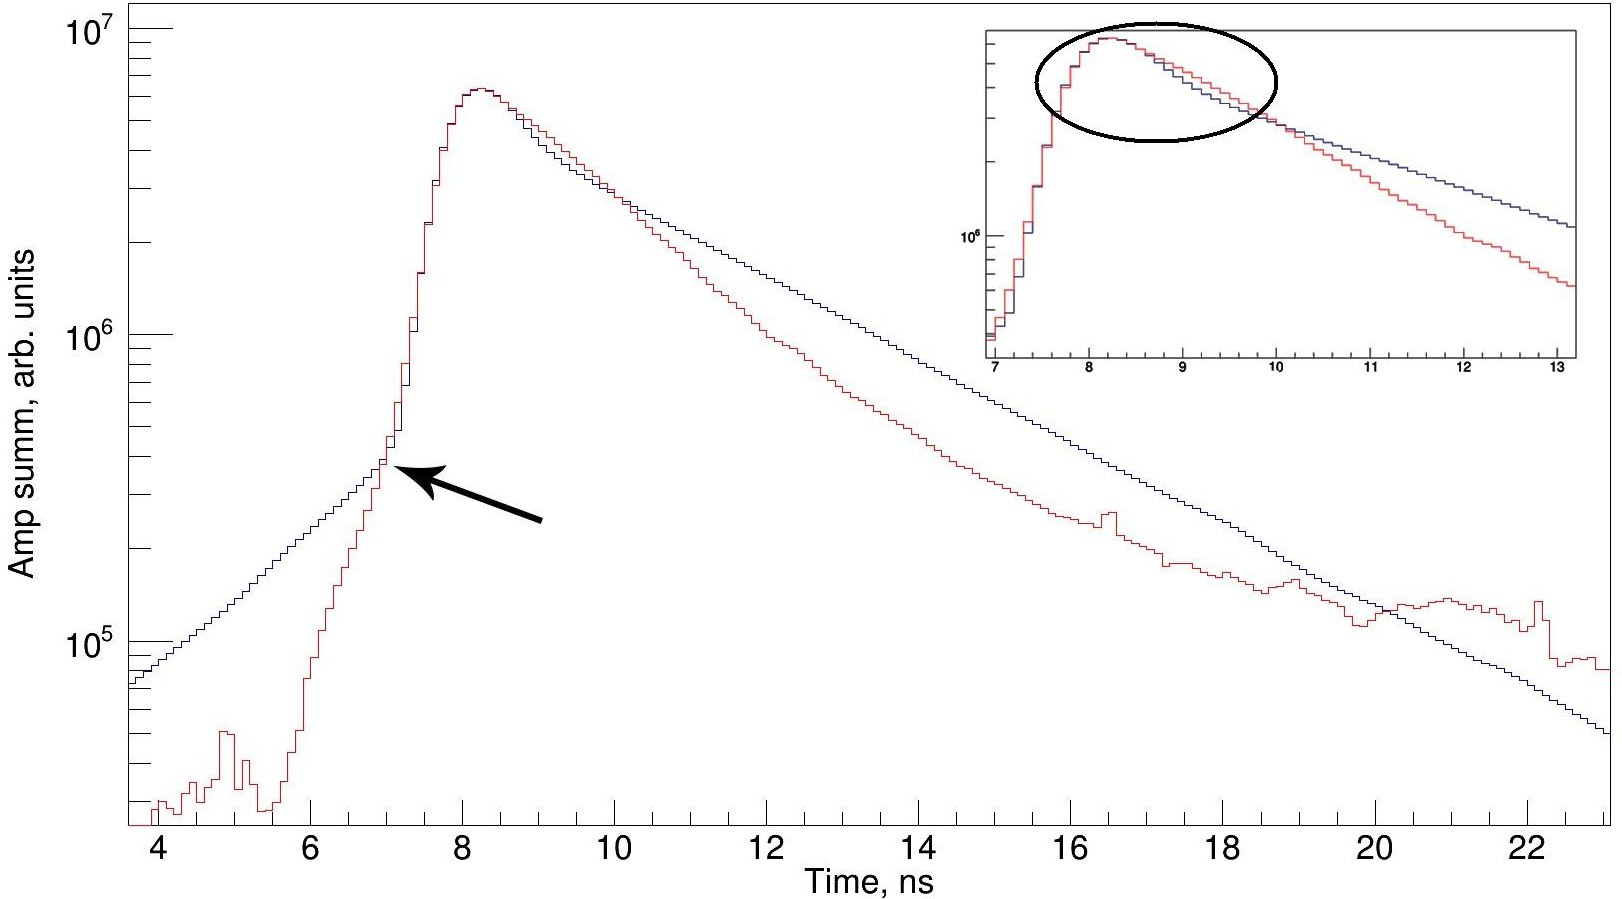
\includegraphics[width=0.68\linewidth]{summ1.png}
	\caption{Pulse summs obtained in the measurements (red) and simulations (blue) in a log scale.}\label{ris:sum}
\end{figure}

Several algorithms of the data processing were developed and implemented into the \er, for example two discriminators --- Constant Fraction(CFD) and Leading Edge (LED), different event selection filters, alignment and summing up of the pulses, etc. Implemented algorithms allowed us to study the summed pulse and understand qualitatively its basic features. All the algorithms could be applied in the same way to both simulated and experimental data.

%\begin{wrapfigure}{l}{0.54\linewidth}
%	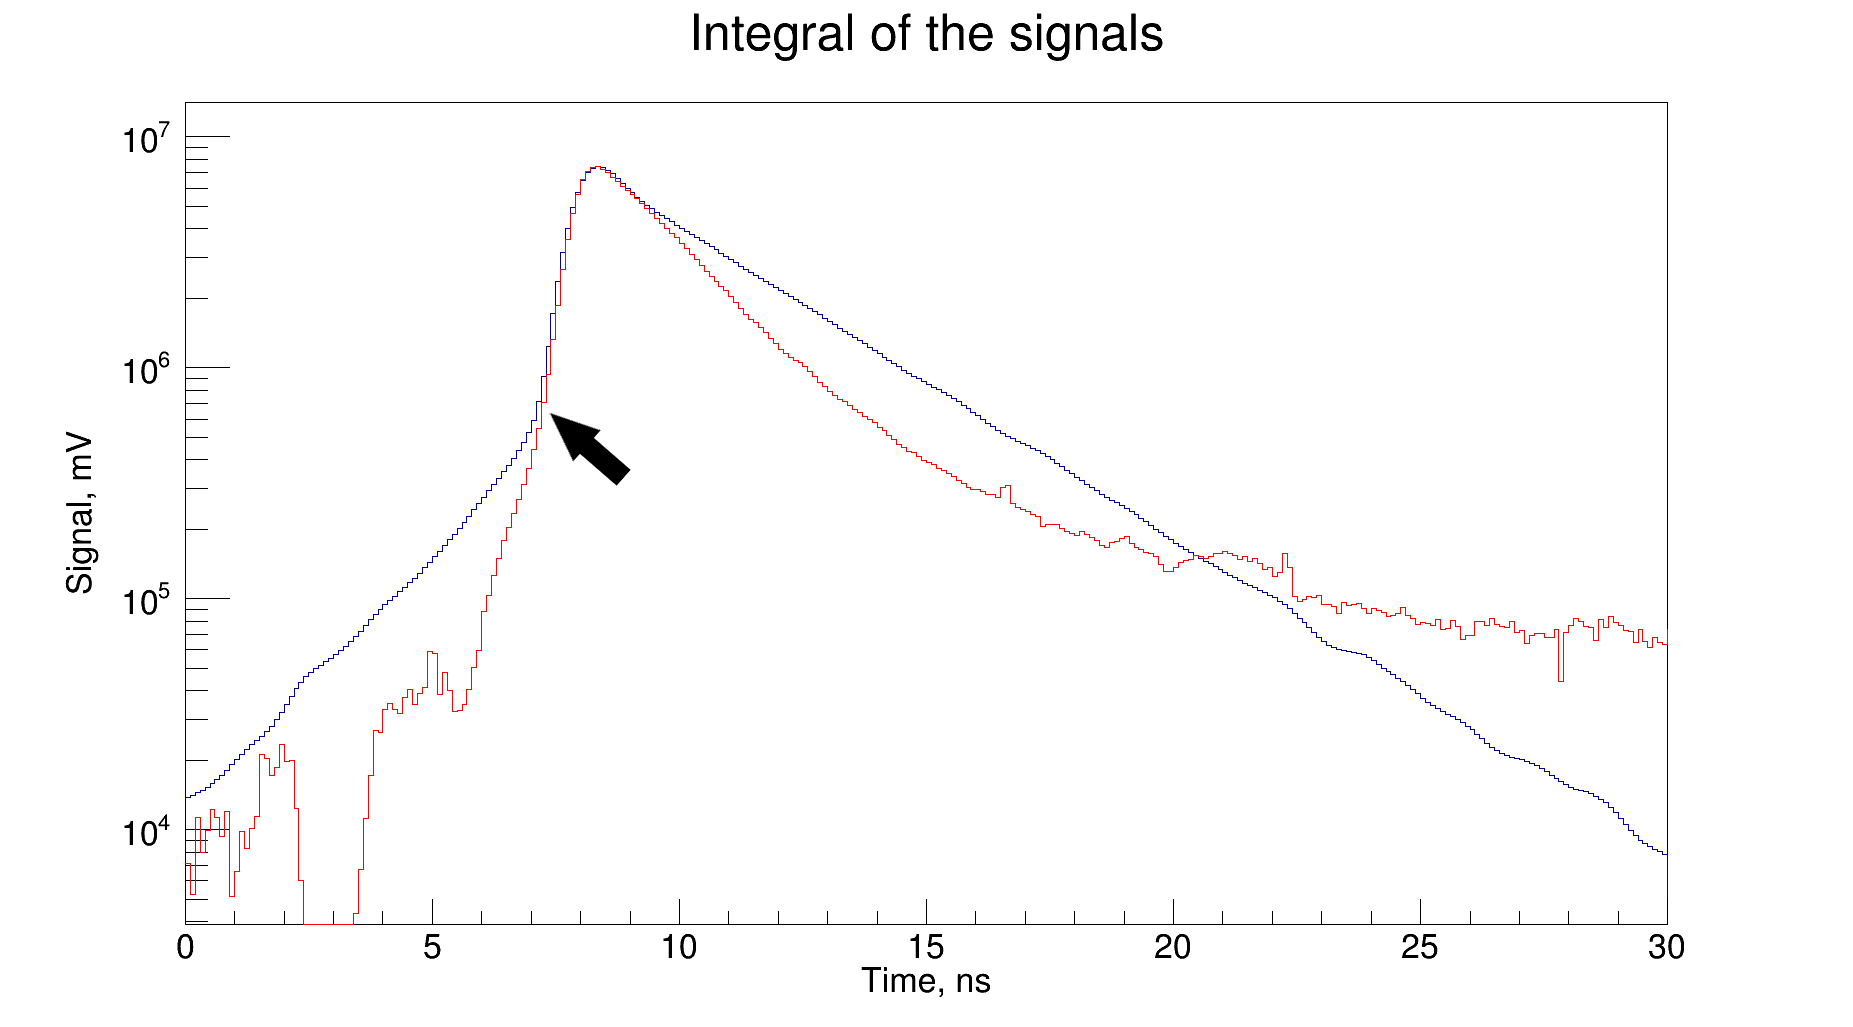
\includegraphics[width=\linewidth]{sum1.png}
%	\caption{Pulse summs obtained in the measurements (red) and simulations (blue) in a log scale.}\label{ris:sum}
%\end{wrapfigure}

Simulated and experimental summed pulses are shown in the Fig.\ref{ris:sum}.
The trigger threshold for the simulated data was set to the 0.77 of the average single photoelectron amplitude.
Such a threshold allowed to match the vertical position of the sharp bend (indicated with an arrow in the picture) in the both pulses. \red{Looking into this figure we are observing the following.} The experimental pulse has the decay profile which includes a fast exponent, faster than the value from the data-sheet, followed by the long non-exponential tail. For simulated pulse there is a bump before the exponential decay (circled in black). This feature is getting more prominent if the light losses at the optical interface go down or cross talks go up. In order to get the quantitative fitting of the parameters and validation of the Monte Carlo model further measurements are needed. It is necessary to use the readout lines tested for their own performance with a fast laser and to read out bigger number of pixels at the same time in order to study all the effects more carefully.

\section{Conclusion}
		
	First small-size prototype of the NeuRad detector was investigated using
	$\gamma$-source. Signal shapes have been obtained using waveform digitizer; timing properties have been studied with specially developed methods of digital pulse processing. The processing algorithms are implemented into the EXPERTroot software package. All measurements were simulated using \er. It was found that the results of the tests and simulations are in a qualitative agreement. Influence of principal parameters of the detector on the pulse shape are understood. For better understanding of the timing properties and \red{quntitative} validation of the Monte Carlo simulations it is necessary to conduct new measurements with the  NeuRad prototype recording bigger number of channels and using well calibrated readout lines.
	The results of this kind of study will allow a correct choice of the optimal readout electronics for the entire system.
	
	%Prototype of the NeuRad detector was investigated for the timing properties.
	%Standard algorithms for signal processing were implemented into the \er\ framework. The simulation of the MAPMT's time response was developed and implemented as well.
	
%	The time resolution of the prototype turned out to be 2.8\,ns which corresponds to 56\,cm of coordinate resolution.
	
%	All measurements were simulated using \er.
	%It was found that the results of experiment and simulation are in a good agreement and it was confirmed that the \er\ options allow to identify the most important effects affecting the timing properties of the intended NeuRad detector.
	%Therefore, the results of this work are very important contribution to the development of the EXPERT project.
	
\section{Acknowledgement}
This  work was partly supported by Helmholtz Association under grant agreement IK-RU-002, RSF 17-12-01367 grant and MEYS Projects (Czech Republic) LTT17003 and LM2015049.

	
\begin{thebibliography}{99}
	\bibitem{ufn} 
	L.Grigorenko et al., “Studies of light exotic nuclei in vicinity of neutron and proton drip-lines at FLNR JINR” Phys. Usp. 59 321–366 (2016); DOI: 10.3367/UFNe.0186.201604a.0337
	
	
	\bibitem{tdr} 
	Technical Design Report of the EXPERT setup of the Super-FRS Experiment Collaboration, https;//edms.cern.ch/document/1865700
	
	\bibitem{diplom} 
	M. Winkler et al., The status of the Super-FRS in-flight facility at FAIR, Nucl. Instr. and Meth. in Phys. Res. B 266 (2008) 4183.
	
	\bibitem{IMexpert} 
	Geissel, H., Kiselev, O., Mukha, I., et al., "Expert (exotic Particle Emission and Radioactivity by Tracking) Studies at the Super-FRS Spectrometer", 2015, Exotic Nuclei: EXON-2014 - Proceedings of International Symposium.
	
	\bibitem{report}
	D. Kostyleva et al., GSI Scientific Report 2016 171 (2017), DOI:10.15120/GR-2017-1
	
	\bibitem{er}
	http://er.jinr.ru/
	
	\bibitem{hm} 
	www.hamamatsu.com/
	
	\bibitem{crystals} 
	https://www.crystals.saint-gobain.com/
	
	\bibitem{geant4}
	http://geant4.cern.ch/
	
%%	\bibitem{petsys}
%	http://www.petsyselectronics.com/web/
	
\end{thebibliography}

\end{document}